\RequirePackage{etoolbox}
\documentclass[a4paper,man,natbib,floatsintext]{apa6}

\usepackage[english]{babel}
\usepackage[T1]{fontenc}
\usepackage[utf8x]{inputenc}
\usepackage[T1]{fontenc}
\usepackage{amsmath}
\usepackage{graphicx}
\usepackage[colorinlistoftodos]{todonotes}
\usepackage{hyperref}
\usepackage{apacite}
\usepackage{verbatim}
\usepackage{csvsimple}
\usepackage{enumitem}
\usepackage{multirow,booktabs,setspace,caption,siunitx}
\usepackage{tikz}
\usepackage{siunitx}
\usepackage{pdfpages}
\usepackage{longtable}
\usepackage{etoolbox}
\usepackage{environ}

\newtoggle{bibdoi}
\newtoggle{biburl}
\makeatletter

\undef{\APACrefURL}
\undef{\endAPACrefURL}
\undef{\APACrefDOI}
\undef{\endAPACrefDOI}

\long\def\collect@url#1{\global\def\bib@url{#1}}
\long\def\collect@doi#1{\global\def\bib@doi{#1}}
\newenvironment{APACrefURL}{\global\toggletrue{biburl}\Collect@Body\collect@url}{\unskip\unskip}
\newenvironment{APACrefDOI}{\global\toggletrue{bibdoi}\Collect@Body\collect@doi}{}

\AtBeginEnvironment{thebibliography}{
 \pretocmd{\PrintBackRefs}{%
 \iftoggle{bibdoi}
  {\iftoggle{biburl}{\unskip\unskip doi:\bib@doi}{}}
  {\iftoggle{biburl}{access from \bib@url}{}}
 \togglefalse{bibdoi}\togglefalse{biburl}%
 }{}{}
}



\usepackage{tabularx} 
\usepackage{longtable}
\usepackage{threeparttablex}
\usepackage{booktabs}
\usepackage{rotating}
\usepackage{pdflscape} 
\usepackage[misc]{ifsym}
\usepackage{csquotes}
\usepackage{lipsum}


\DeclareCaptionLabelSeparator*{spaced}{\\[2ex]}
\captionsetup[table]{textfont=it,format=plain,justification=justified,
 singlelinecheck=false,labelsep=spaced,skip=0pt}
\captionsetup[figure]{labelsep=period,labelfont=it,justification=justified,
 singlelinecheck=false,font=doublespacing}


\title{A comparison of eye movement on perception and imagination: A multivariate pattern analysis approach showing importance of spatial information.}

\shorttitle{MVPA of eye movement on perception and imagination}
\author{Mirko Bristle}
\affiliation{
Division of Cognitive Psychology, Perception and Research Methods\\
Department of Psychology\\
University of Bern }
\note{
Supervised by Lilla Gurtner and Dr. David Weibel\\

\vfill
author note\\
All code is available at \href{https://github.com/MBristle/Forschungsatelier}{github.com/MBristle/Forschungsatelier}.
Access must be requested in advance.
\begin{flushleft}
Mirko Bristle\\
Gemmistrasse 22\\
3604 Thun\\
E-Mail: \href{mailto:mirko.bristle@students.unibe.ch}{mirko.bristle@students.unibe.ch} \\
Matrikelnummer: 14-109-573

\newpage
\end{flushleft}}

\abstract{
We imagine the world similar to how we perceive it. This similarity is consistent and robust over time. While decoding analyses have been used to classify patterns of perception especially in brain imaging, to our knowledge no study to date has compared imagination and perception based on eye movement. The aim of this study was to show improved classification scores based on spatial information compared to summary information for perception, imagination and the transfer. We conducted a perception-imagination task with 15 images belonging to one of three categories (art, landscape, faces). Participants (n = 5) looked 15 sec at a picture and afterward imagined each image for 15 sec. This was 30 times repeated for each picture. We used a linear support vector machine to perform the classification analysis. A leave-one-out approach was applied for cross-validation. The results show that the overall classification of perceived and imagined images is above chance level for spacial information and superior to summary information. Training on perception data and cross-validating with perception data lead both independently to increased classification. The classification accuracy depends also on the picture category. Overall we show a new approach of spatial pattern classification in eye movement for perception and imagination data. 
}

\begin{document}


\maketitle
% Einleitung
When observing our environment, the gaze pattern plays a crucial role in constructing a mental representation and is influenced by cognitive processes\citep{Hayhoe2005}. At the same time, mental imagery defined as the representation and the concomitant sensational experience in absence of external stimuli, are closely related to perception. Both processes share the same biological processes and because of this, mental imagery can affect perception and the other way around. \cite{Winawer2010} were able to produce a motion aftereffect from the visual imagery of motion. This adaption transfer shows that mental imagery alters neural pathways which are at a low-level of the neural signal processing in a typical sensory-specific area.\\
This close relationship exists not only for simple low-level phenomena but also for several learning-paradigm, such as the line bisection task. Participants get better in classifying whether a single line in between two lines lies closer to on side or the other \citep{Tartaglia2009}. In the same way, imagend associative learned material produced the same emotion-evoking response as perceived material\citep{Lewis2013}. These effects can be of clinical relevance for people with several different psychological disorders such as post-traumatic stress disorder (PTSD), anxiety disorders, bipolar disorder and schizophrenia \citep{Holmes2010}.
Multiple brain imaging studies have tried to track down the interplay between perception and imagination. Already on very low-levels of neural processing such as the visual area 1 (V1)  were similar activation patterns when imagine or perceiving simple objects such as bulbs \citep{Bergmann2016}. Similarly, stimuli could be discriminated using multivariate pattern classifiers in low-level areas such as  V1 and V2, even though the activation pattern was much lower for imagery \citep{Cichy2012, Lee2012}. Climbing up the visual hierarchy, the resemblance increases more and more \citep{Stokes2009}. This observation overlaps with the idea that higher level areas such as the medial temporal lobe (MTL) are more associated with memory encoding and retrieval \citep{Reddy2010, Johnson2014}. \\
These recent findings can very well be integrated into older research on eye movement. For instance, \cite{Laeng2002} asked participants to observe an irregular checkboard or color images and afterward to imagen them with their eyes open. One condition was requested to fixate the center of the screen during perception, a second condition during imagination and a third had no limitations in exploring the stimuli. They revealed that the sequential order of the eye movement was similar during perception and imagination and that the fixated gaze condition during perception produced the same pattern in imagery. These findings agree with findings where participants first viewed and afterward imagined a complex picture or constructed them from verbal description \citep{Johansson2006}. Interestingly, these findings are not only functional to the retrieval right after encoding, but the prolonged fixation patterns on the areas where the stimulus has been persisted over one week \citep{Martarelli2013}. \\
Generally speaking, eye movements can be described by different measures (fixations, saccades, blinks, their durations, pupil and coordinate). So far most of the analysis in the field of perception - imagination research focused on the coordinate of the fixation. More advanced techniques were introduced to investigate spatial distributions, scan-paths by looking at string-based and geometric comparisons or probabilistic approaches \citep{Coutrot2018a}. Each technique on its own is able to answer a specific question and model a certain part of the eye movement behavior. In a diagnostic analysis, a high level of previous knowledge is needed to interpret the full spectrum of information. \\
In this context, multivariate pattern analysis has the advantage of learning a model from the data based on a sample dataset. Not much research has been done to perform multivariate prediction on eye movement and to our knowledge up to date, no research investigated these techniques in the field of perception and imagination with eye tracking data. 
The aim of this study is to perform a prediction analysis by classifying images based on their gaze pattern. Therefore we propose that each picture has a unique pattern of contemplation. Further, we want to replicate the importance of spatial information and so the importance of feature selection for the perception and imagination debate. Therefore we compare the performance of simple summary information to spatially distributed information. We hypothesize that this spatial gaze pattern exists not only when perceiving an image but also when imagining one. As mentioned above the pattern during imagination should be functional depending on perception and therefore a classification of imagined pictures based on information of perceived images and vice versa should be above chance level.


%%%%%%%%%%%% Methode %%%%%%%%%%%%%%%%
\section{Methods}

\subsection{Participants}
In this experiment, five participants were recorded (four female). They were all enrolled at the University of Bern and had experience in psychological testing. Their age varied from 24 to 28 years ( mean 25.25; SD 1.89) and all participants reported normal or corrected-to-normal vision. They were not paid for participation. The Experiment was permitted by the ethical review board of the Faculty of the Human Sciences at the University of Bern, Switzerland. All participants gave informed consent on their participation according to the Declaration of Helsinki and were aware that they could end the experiment at any time.\\

\subsection{Stimuli} 
The images were split into three different picture categories (landscape, art, faces). Each category was assumed to lead to a specific eye movement pattern \citep{Anderson2013, Henderson2003} but also each picture should have a specific eye movement pattern. In total 15 pictures have been used, having 5 pictures in each of the three categories. The images were selected by the experimenter after pioloting, including pictures with a high number of fixations and a high variance in fixation location. All images had a resolution of 1280 x 1024 pixel and were presented in RGB color. Face images originated from a dataset of the European Conference on Visual Perception \citep{Hancock} and contained four female and one male face. Each face was presented in front of a blue background, which was extended to match the size of the other images. Due to this most fixations should fall into a central part of the screen where eyes, nose, and mouth are located \citep{Hernandez2009}. Both, the landscape and the art pictures were retrieved from the internet. Criteria for the landscapes were that they contained no human being or animal and had a uniform sky in the upper half of the screen containing no clouds or other objects. Considering this fact, most information should lie in the bottom of the screen and therefore most fixations should be located around this area. Finally, art pictures contained a set of human beings distributed over the whole picture. Since salient features were spread all over the screen, we expected as well the fixation to be spread all over the screen (FIG sample screen). \\

\subsection{Apperatures} 
Eye movements were registered using the EyeLink 1000 Software, which was provided by SR Research GmbH (Canada). The samples were recorded at 500 Hz binocularly. Using an infrared light sensitive camera, the eye tracking device was able to track the gaze on the image by calculating the position from the corneal reflex and the pupil location. For calibration, we used a 9 point grid presented at the beginning of the experiment on the screen. After each trial, a drift correction was applied by looking at a central point on the screen. The participants were seated in front of a table, facing the eye tracking device and the display. The participants rested their chin on a head support and faced the 26-inch Display. The Distance between the eyes and the display was approximately 75 cm. \\

%Psychopy

\subsection{Procedure} 
\begin{figure}
\centering
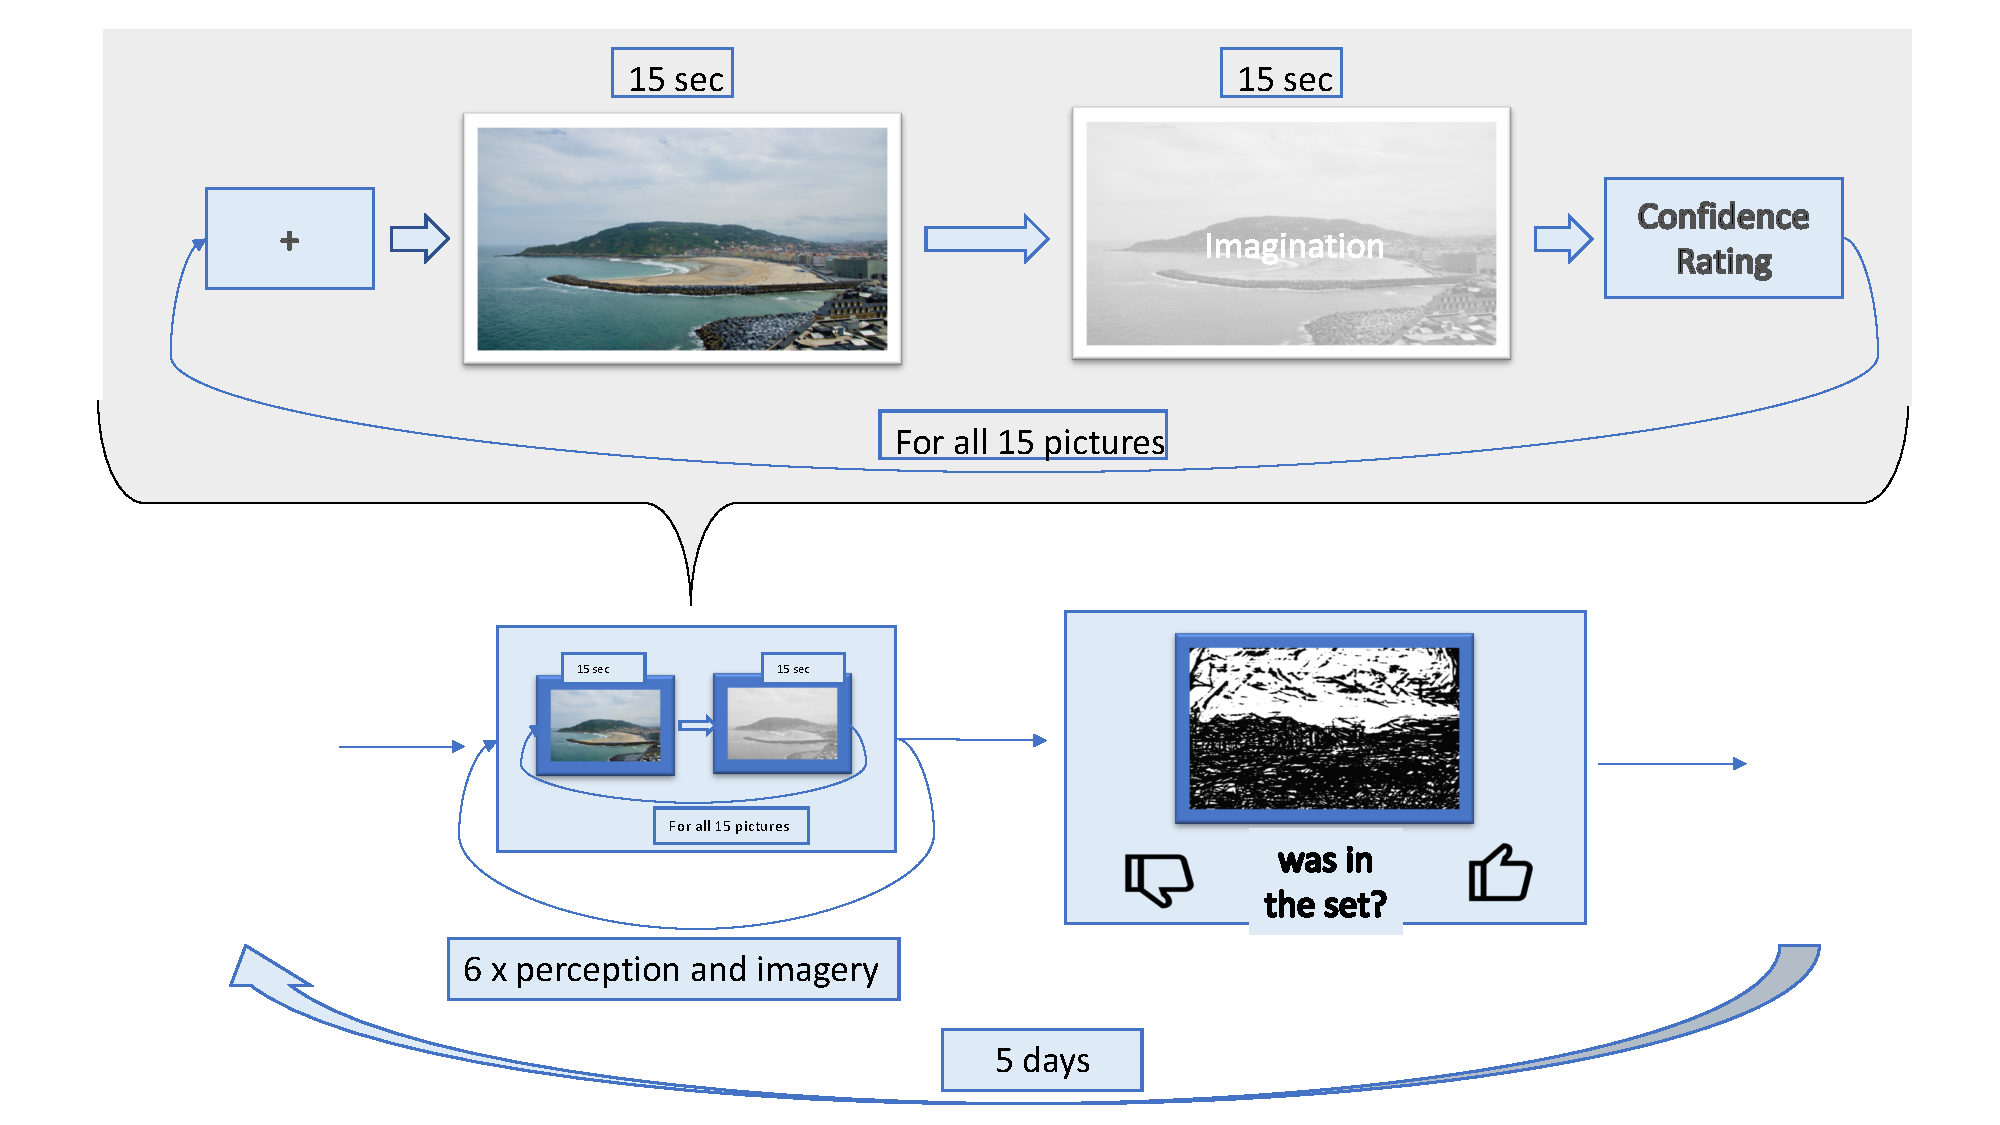
\includegraphics[width=1\textwidth]{Procedure.pdf}
\caption[Procedure]{\label{fig:Procedure} Design of the study. Each trial started with a fixation-point followed by a 15 seconds of picture presentation, followed by 15 seconds to imagine the seen image while still looking at the screen. At last, a confidence rating was obtained to judge how well the participants were able to imagine the image. \\ This procedure was repeated for each of the 15 images in all six blocks. At the end of each session a discrimination task was performed. There were 5 sessions per participant. }
\end{figure}

The experiment was programmed on EyeLink 1000 Software of the eye tracker itself. It was split into five sessions each containing six Blocks of the fifteen pictures. Pictures were randomly shuffled for each session. 
The participants were asked to complete one session a day under the supervision of the experimenter. After calibrating and validating the eye tracking device the task was started.\\
At first, participants were presented with a fixation point for a jittered time span (1-5 sec), followed by the instruction to explore the picture for 15 seconds and then to try to imagine the same picture for another 15 seconds. Participants were asked to keep their eyes always on the screen when perceiving and imagining the picture. After 15 seconds of imagination, the participant was asked to perform a confidence rating on how well he was able to imagine the image. This procedure was repeated for each image in each block at random order. Participants were free to take a break in between the trials if they felt tired (median overall sessions was 2; see fig.\ref{fig:Procedure}). 
To improve the motivation we performed a control experiment at the end of the last presentation of each session. Here we presented the fifteen pictures known from the session before as well as fifteen pictures which were new to the participant. Following the procedure of a yes-no identification task, the participant had to judge whether the seen picture was in the set of observed pictures or not. Each picture was partially covered with random noise of 1500 blocks. The size was always a square and was drawn from a normal distribution with 30 px in mean and 7.5 px standard deviation. After a fixation cross with a jittered time interval (0.5-1 sec), the Stimuli were presented for 40 ms and backward masked by three images each presented for 10 frames. Each masked consisted of 5000 blocks with their size drawn from a normal distribution with mean 10 px and a standard deviation of 2.5 px. All masks presented during and after the stimulus were load in advance during the fixation cross of the current trial. After the mask, the participant had to make their judgment. This procedure was repeated for all 30 images in random order. This control-experiment was not further evaluated.\\

\subsection{Analysis} Eye-tracking data was recorded on the EyeLink 1000 software and aggregated in Matlab 2015b \citep{Mathworks2015}.  The calculation of fixations and blinks were performed online on the EyeLink 1000 software. All further analyses were calculated offline in Python 3.7 \citep{Python2018}. Additionally, the "Sklearn" package \citep{Pedregosa2012b} and "SciPy" \citep{Oliphant2007} were used. % Packages angeben
As measures of the fixation, we used X and Y coordinates of the right and left eye, the duration of the fixation, whether the measure was surrounded by a blink and the number of fixations per picture. We excluded the pupil dilatation as a measure since the luminance of the pictures was not controlled what could influence the results heavily.\\

\subsubsection{Feature extraction}
Two feature sets were generated to compare between the performance on summary-features and advanced spatial features. 
The summary feature set contained 6 features: mean coordinate of the right and the left eye ($X_{right}, Y_{right}, X_{left}, Y_{left}$) of the trial and the number of fixations and the number of blinks in the trial. \\
As spatial feature set, we split the fixation into 36 bins. The size of the bins was estimated by quantile-base discretization of the data. For each subject and condition (perception/ imagination) the abscissa and ordinate were split into six parts, all having the same amount of fixations in each part. This gives an interpretable space and takes more dense areas (as the middle) into account. The number of bins was chosen by cross-validated performance on the perception and imagination data. For comparison, the mean of the two was chosen as an optimal number of bins. % evtl noch abbildung und beschreibung wieso 6 bins
As a feature set for the spatial data, for each bin the fixations were summarized into aight features. 
 \begin{enumerate}
\item The proportion of fixations on this bin compared to all fixations in this presentation period. 
\item The absolute number of hits on the bin during the presentation period.
\item The proportion of fixations on the bin of the left eye compared to all fixations of the left eye during this presentation period.
\item The proportion of fixations on the bin of the right eye compared to all fixations of the right eye during this presentation period. 
\item The mean duration of the fixation of this bin during this presentation period.
\item The mean temporal position of the fixation of this bin during the presentation period.
\item The mean number of blinks surrounding the fixations in the bin during the presentation period.
\item The absolute number of blinks surrounding the fixations in this bin during this presentation period.
\end{enumerate}
Missing data was excluded from all features (summary data 1.24\% and spatial data 0.43\%). Further, we excluded fixations which were not in the area of the picture on the screen. \\

\subsubsection{Prediction analysis}
Compared to the modeling approach, where the goal was to find the best fitting model, the goal in this analysis is to predict the data as good as possible. Therefore the toolbox of supervised learning algorithms was considered. At first, a classification problem was specified. The aim was to minimize the error between the predicted picture and the actual picture.  While the current state of the art techniques summarized as deep learning have a huge number of parameters to tune and are in need of a big dataset and computational power, older sophisticated techniques were preferable for smaller datasets such as the one conducted in this experiment. From the literature, it is known that support vector machines (SVM) perform well on classification problems, such as recognition of handwritten letters or faces \citep{Bahlmann2002,Guo2001}. Today SVMs are used in clinical settings for analyzing magnetic resonance imaging data. Compared to deep learning using artificial neural networks, a major advantage of this technique is that SVMs have a certain degree of interpretability and work well on rather small datasets \citep{Segovia2010}.


For this analysis, a linear SVM was chosen.  The goal of the classifier is to predict a test dataset based on the trained model as good as possible. This is achieved by maximizing the margin of a hyperplane between two classes. A support vector machine is defined as the following optimization problem: 
\begin{align}
\text{argmin}_{w,b,\epsilon} &\qquad \frac{1}{2} w^Tw + C\sum^k_{i=1} \epsilon_i \\
\text{subject to }&\qquad   y_i(w^t\phi(x_i)+b) \geq 1-\epsilon_i, \\ & \qquad \epsilon_i \geq 0, \qquad C>0,
\end{align}
given pairs of training data $X_i$ and the corresponding labels $y_i$, $i=1,...,k$, where $X_i \in R^n$ and $y_i \in \{1,-1\}^k$. Even though mappings of $x_i$ to a higher space are possible by the function $\phi$, in this work only linear mappings were considered to reduce overfitting. C is the penalty parameter of the regularisation term $\epsilon$, which can be interpreted as the error term. C was set to 1 in all analysis \citep{Cortes1995}. \\
As labels $y_i$ the fifteen pictures described above were used. Since the original SVM can only perform binary classification, a one-class-against-rest-classification was performed. This provides an estimate of how good the particular picture can be discriminated from all other pictures.\\ %paper dass dies besser ist als andere 
To avoid dominance effects of single features, the training and test data were scaled by a Min-Max-Scalar trained on the training data.\\

To evaluate the model performance leave-one-group-out cross-validation was applied. Similar to k-fold cross-validation the data of one participant was taken as test data and the rest of the data was used to train the SVM. This procedure had the advantage of controlling the risk of subject depending gaze patterns and reducing overfitting. As simple accuracy scores are not well suited to evaluate signal detection problems, since they depend on the criterion of the observer (in this case the SVM)  and neglect rates of false positive and true negative observations, the receiver operating scale was calculated and the area under the curve was used as measure of class discrimination \citep{Hsu2010}.\\ 

\subsubsection{Modeling of accuracy}
In order to confirm that the classification is above chance level, the data was bootstrapped overall AUC scores for summary-features and for spatial-features. The bootstrap had 5000 iterations each time selecting a random sample set. This procedure provides an estimate of the distribution of the mean of the data. 95\% confidence intervals were calculated. To be above chance level, the distribution has to be above the AUC value of 0.5.
To evaluate the model performance on the different features a Bayesian hierarchical multilevel model was used.  All models were calculated in R \citep{RDevelopmentCoreTeam2016} with the package "brms" \citep{buerkner2016brms}. All priors were uninformative half-student priors. The distribution of the data was assumed to belong to a gaussian-family.\\
First, the group level effects of participant and pictures were entered into the model. Followed by the population effects of category (Face, Art Landscape), training - test comparison and feature type (summary / spatial) and all interactions between them. All models had 1000 warm up samples and 1000 iterations with four chains. 
To reduce the risk of overfitting, leave-one-out cross-validation (LOO) was performed using a backward stepping approach. This means each predictor and interaction was once removed and then compared to the full model described above \citep{Vehtari2016}. The full model was defined as superior to a more economical model if the LOO value was higher than the one of the more economical models plus the standard error (SE). All effects will be reported with the credibility interval (CI) of 95 \%. 


\section{Results}

\begin{figure}
\centering
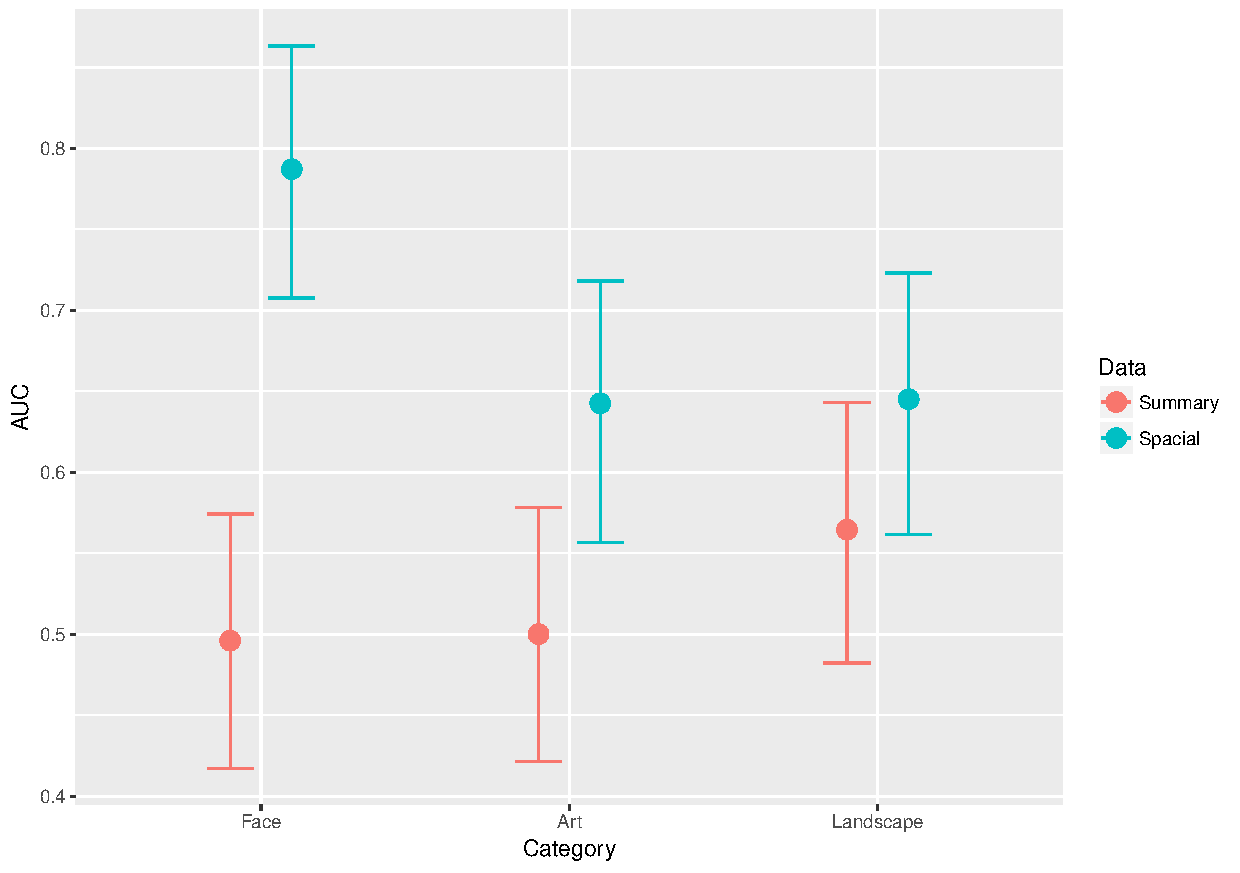
\includegraphics[width=1\textwidth]{CategoryXFeature.pdf}
\caption[Category $\times$ Features]{\label{fig:CategoryXFeature} Performance of SVM measured as area under the curve (AUC) of the category $\times$ features interaction trained on imagination and tested on imagination. This training-testing condition is expected to classify the worst. We see that the credebility intervals of the summary data are never above chance. On the other hand all spatial features surpass the chance level. The increase of accuracy for the category face from summary features to spacial features is higher than the same for art. Landscape benefits the least from the spacial information. }
\end{figure}
\begin{figure}
\centering
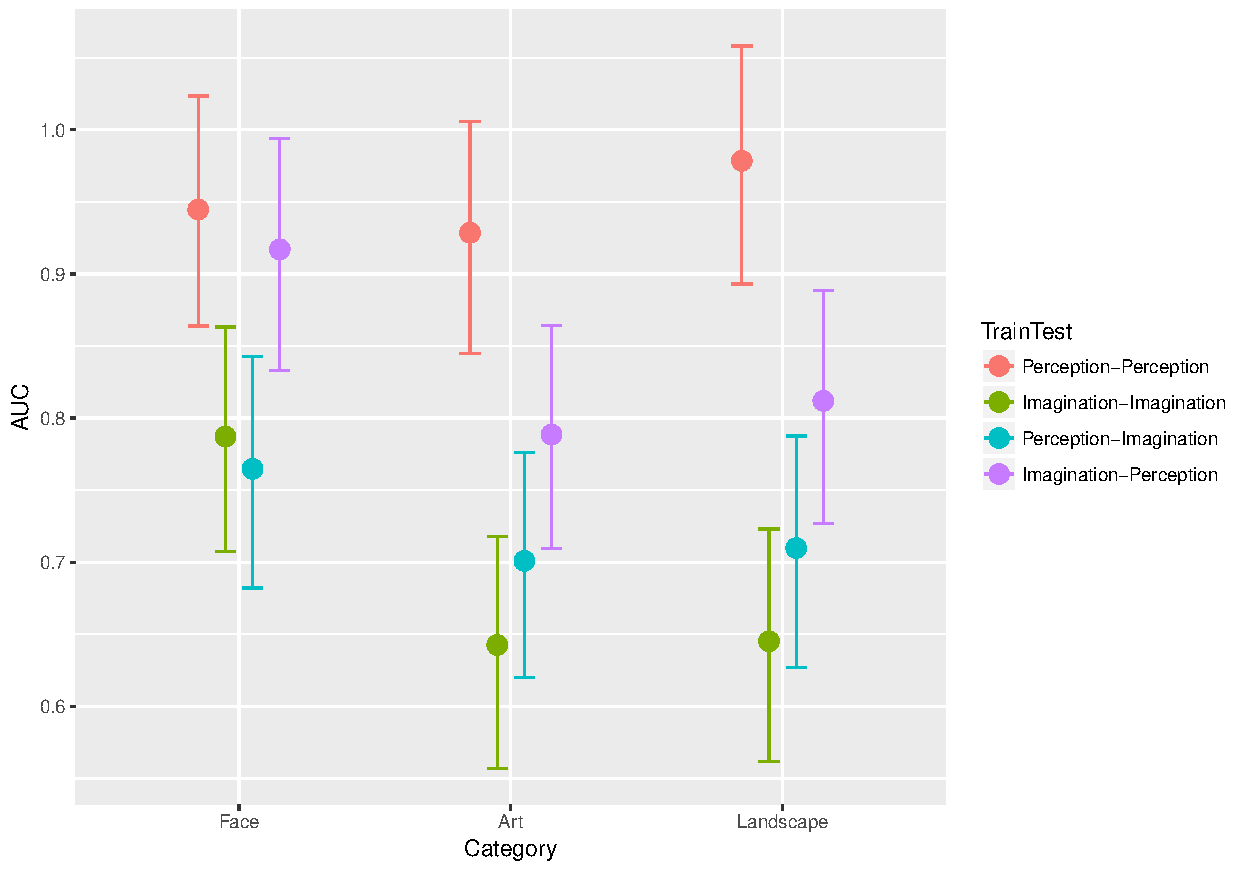
\includegraphics[width=1\textwidth]{CategoryXTrainTest.pdf}
\caption[Category $\times$ Training-Test-Condition]{\label{fig:CategoryXTrainTest} Performance of SVM measured as AUC of the category $\times$ training-test-condition interaction for spacial features. Training and cross-validating the SVM on perception performs with the highest AUC.    A classifier trained on imagination and tested on either imagination or perception has an increased performance of faces compared to art pictures. Landscapes don't differ from art.}
\end{figure}
\begin{figure}
\centering
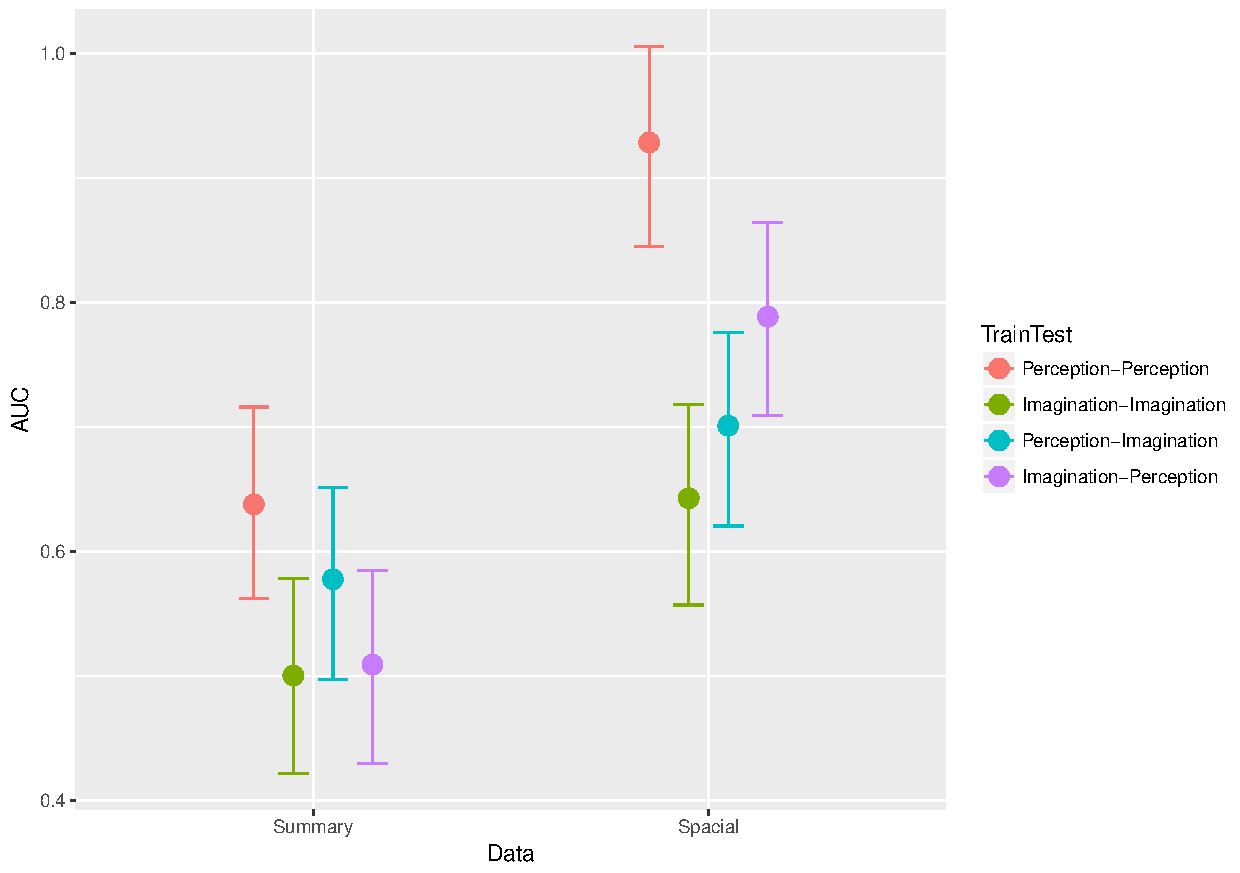
\includegraphics[width=1\textwidth]{FeatureXTrainTest.pdf}
\caption[Training-Test-Condition $\times$ Features]{\label{fig:FeatureXTrainTest} Performance of SVM measured as AUC of the training-test-condition $\times$ features interaction for art pictures. For summary features only the SVM trained on perception and tested on perception passes with a CI of 95\% Chance level. On the other side, all spacial features are classified above chance. For spacial features both SVMs tarined on imagination and perception but tested on perception are higher than the two SVMs tested with imagination. } 
\end{figure}

All participants were included in the analysis. One block was excluded from all participants and sessions because of data loss. One participant aborded a trial before it was finished. The all other pictures in this block were excluded as well from the analysis to keep a balanced design.
After training the SVM the cross-validations scores of the AUC were bootstrapped and entered into a Bayesian multi-level model.
That classifier performed on average above chance level. Performance above chance is  defined as a performance of a AUC of greater than 0.5. Both summary features and spatial features were bootstraped seperatly. Both were above chance, with the difference that spatial features ($M$ 0.81, CI[0.78;0.82]) performed better than the summary features ($M$ 0.55, CI[0.54;0.58]). \\

For the bayesian multi level model, the full model was specified as described above and backward elimination of predictors was performed. First group level effects were optimized and then population level effects were analysed. \\
Both group level effects subject ($\Delta_{LOO(full - full_{-subject})}$ -13.72 [SE 8.15]) and image ($\Delta_{LOO(full - full_{-image})}$ -54.18 [SE  14.89]) were predictors of the prediction accuracy of the SVM. 
On the population level, the model without the three-way-interaction (f\_3WI) was superior ($\Delta_{LOO(full - full_{-f\_3WI})}$ 5.37[SE 5.33]) to the full model.  All three two-way interactions turned out texplain a relevant part of variance compared to the model without the three-way-interaction (
Category $\times$ feature-type $\Delta_{LOO(f\_3WI - f\_3WI_{-Category \times feature\_type})}$ -60.93 [SE 16.84]; 
Category $\times$ train-test $\Delta_{LOO(f\_3WI- f\_3WI_{-Category \times train\_test})}$ -15.94 [SE  9.43];
feature-type $\times$ train-test $\Delta_{LOO(f\_3WI- f\_3WI_{- feature\_type\times train\_test})}$ -44.29[SE  13.09]).
This final model converged with six diverging transitions. For all parameters $\hat{R}$ was smaller than 1.01, no parameter had a Monte Carlo standard error greater than 5\% of the posterior standard deviation and the effective sample size was for all parameters greater than 10\% of the total sample size.\\

In the final model, the proposed effect of better accuracy for spatial features compared to summary statistics ($\Delta$mean -0.147, CI[0.032;0.211]) was observed. 
In general the classification for landscape pictures ($\Delta$mean 0.003, CI[-0.092;0.033]) was not higher or lower than art pictures but both were less accurate than faces ($\Delta$mean 0.145, CI[0.047;0.176]). 
The posterior distribution of the AUC trained on perception and cross-validated on perception ($\Delta$mean 0.287, CI[0.224;0.308]) was higher than any of the three other combination of training and testing data. 
Training on imagination and testing on perception ($\Delta$mean 0.147, CI[0.084;0.168]) was classified more accurate than both training on perception ($\Delta$mean 0.059, CI[-0.003;0.079]) or imagination and cross-validating on imagination. \\

The two-way interaction feature-type $\times$ category revealed an increased difference in accuracy between spatial and summary features for faces ($\Delta$mean -0.149, CI[-0.203;-0.097]) compared to art (see fig.\ref{fig:CategoryXFeature}). 
Whereas the difference between spatial and summary features was decreased for landscapes ($\Delta$mean 0.062, CI[0.027;0.114]) compared to art. 

The two-way interaction between category $\times$ training-testing-condition showed an decrease in difference of accuracy between category art to faces when trained on perception and tested with imagination ($\Delta$mean -0.081, CI[-0.156;-0.004]) or perception ($\Delta$mean -0.129, CI[-0.204;-0.054], see fig.\ref{fig:CategoryXTrainTest}). 

At last, looking at the interaction of feature-type and train-test-condition revealed an smaller increase of accuracy between summary-features and spatial-features when tested on perception and trained on imagination ($\Delta$mean -0.139, CI[-0.030;-0.079]) or on perception ($\Delta$mean -0.149, CI[-0.209;-0.088], see fig.\ref{fig:FeatureXTrainTest}).


%\newpage
\section{Discussion}
The purpose of modeling the accuracy of the AUC of the SVM was to invest if and how the spatial feature set improves the accuracy. Knowing the nature of the features and the picture categories, it is possible to interprete how eye tracking is used during imagination and perception. \\
As seen in the bootstrapping analysis the mean accuracy of the summary features is just above chance most probably by the interaction training-testing-condition of perception-perception.
On the other hand, we saw as expected improved AUC classification above average for spatial features in the bootstrapping analysis and the Bayesian multilevel model.
In the context of comparing spatial features to summary features, the higher improvement of the AUC when tested with perception is an important finding. The improvement of perception as training set could be due to the fact that there is less noise in the data since the participant was at all times confronted with the picture and due to this, there was less room for any kind of lapses.
Taking the categories into consideration we saw a higher accuracy for faces, which was driven by the spatial data. Landscapes profited the least from spatial information. These two effects might be due to the properties of the pictures. The summary of the landscapes was maybe slightly more informative since the pictures had their points more distributed especially in the lower half of the picture. Since the special features split the pictures based on their quantiles and for all eye movement data a distribution peaking at the center of the screen can be assumed, information laying in the central part of the screen profited most from the chosen method of picture discretizing. Outer parts of the picture were summarized into bins which contained more pixels, what maked them less informative to small changes. 
The interesting effect of the property of the picture category could also explain the effects of the interaction between the picture category and training-test-condition. Faces had a reduced difference in accuracy between the reference imagery and both conditions trained with perception. This could be interpreted as an increased improvement of the classifier when trained with imagination data for both test sets. \\
An other important difference could be the informative richness of the image. It is highly plausible that a painting has more detailed information, each being represented mentaly as a separate part of the image. This could cause scalings of parts of the image and alter the gaze patterns in the imagery condition which is not expected by the current set of features. On the other hand, faces are more homogeneous which makes each bin of features more informative, since the spatial position has interpretable meaning. \\
Our results confirms the idea that imagination and perception are closely related using novel techinques of multivariate pattern analysis on eye movement data. In this study we showed the importance of spatial resolution for image classification based on the fixations of eye movents during perception and imagination. On the other side the data showes decreased performance for imagination as testing set independend of which training set was used. This could have multiple reasons, which should be investigated by improved feature construction  \citep{Johansson2006, Laeng2002}.

\subsubsection{Limitationen}
There are some limitations which must be considered. Since our study was of an experimental nature only 5 participants were recorded. Even though we cross-validated on a subject level, our classifier might not be generalizable for other participants because of the small sample size. 
An major draw back is, that the brightness, luminanz and contrast of the images were not controlled. The influence was reduced by excluding the pupil from the analysis but it has been shown, that visual awareness influences imagery \citep{Pearson2015}. An other issue was the length of the design. In order to get enough data pictures were repeatedly presented. This might lead to alteration in there gaze pattern, since the content is known to the person. An other problem is the decreased concentration of the participants, since on experimental session lasted one hour. This could lead to decreased data quality especially for imagined data towards the end of each session.

\subsubsection{Future perspective}
In the future, it would be interesting to see whether it is possible for the imagined data to separate the distribution of internal picture representation and lapses.  As seen above, when creating features for eye tracking data the structure of the image needs to be considered and features need to be optimized with respect to this information. 
The presented spatial features chosen in this paper had the purpose of being in some sort similar to the commonly used summary features which could one at the time also be used in a univariate analysis. In future work, advanced features could reveal more whether there is a transformation in the data between imagination and perception. Another interesting question is whether the influence of the increased level of lapses and decreased level of attention proposed in this paper could be decreased.\\
Further should be investigated whether the same accuracy level is achievable with more participants with fewer trials each. This could be beneficial for generalization and as well reduce the problem of repeated presentation of the same image to the same participant. On the other hand the time sequencial change in the gaze behavior might have valueable information in clinical settings.  Overall we propose that once robust features are available, this type of analysis could lead to cost efficent highly accurate individual diagnostics.
%Quellen
% integration literatur

\begin{comment}
GitGud
\end{comment}
\clearpage
\bibliographystyle{apacite} 
%http://www.ctan.org/tex-archive/biblio/bibtex/contrib/apacite/apacite.pdf 

\bibliography{/Users/mirko/Documents/bibTexLibrary/library.bib} 
\newpage
\clearpage
\end{document}

%
% Please see the package documentation for more information
% on the APA6 document class:
%
% http://www.ctan.org/pkg/apa6
%

